\documentclass[a4,12pt]{article} 
\usepackage{graphicx}
\usepackage{xepersian} 
\settextfont{Yas} 
\title{ تکالیف سری دوم کنترل خطی}
\author{یاسمین خورشیدی 40117963}
\begin{document}
	\maketitle
	\section{سوال اول}{
		%	\begin{figure}
			\centering
			%		\textbf{سوال 1 :}
			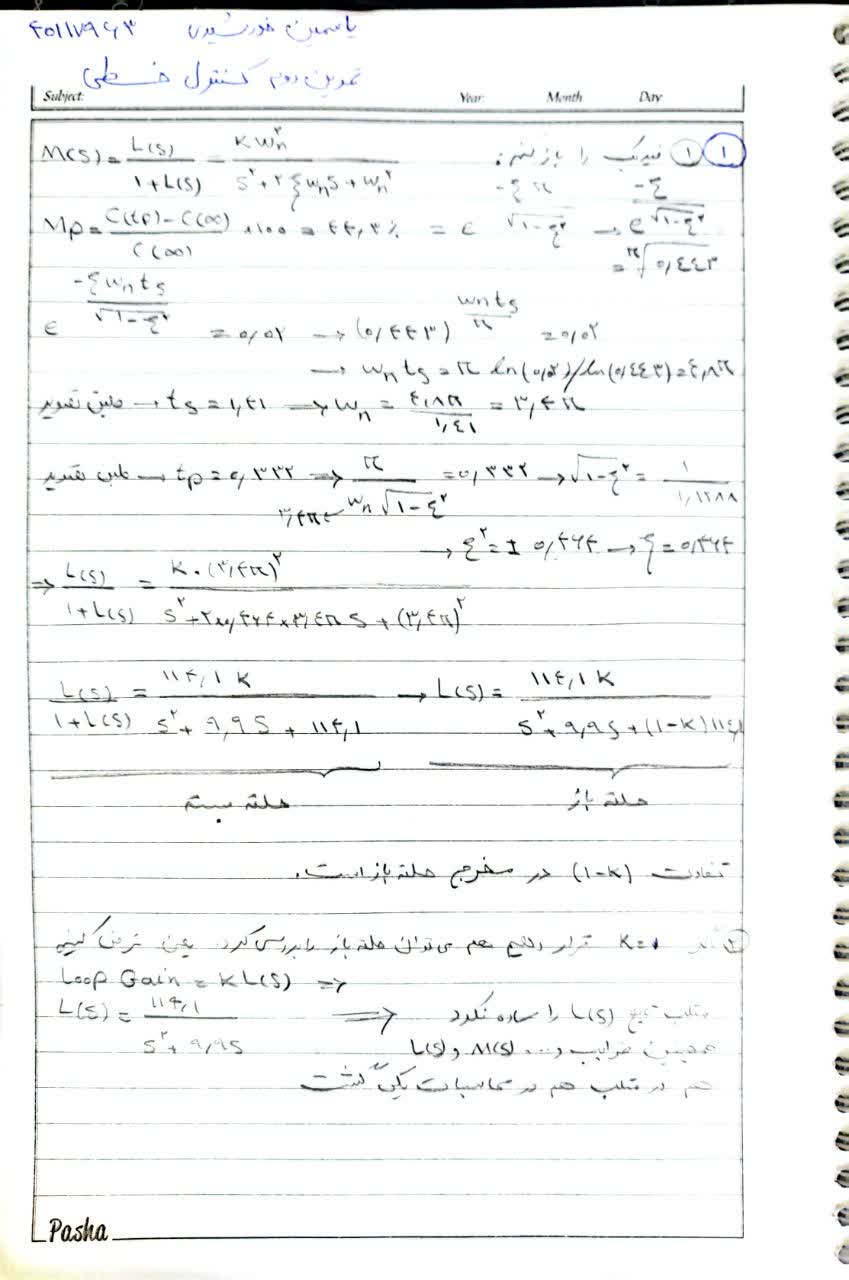
\includegraphics[width=15cm]{h2s1.jpg}
			%	\end{figure}
	}
	\section{سوال دوم}{
		%   \begin{figure}
			\centering   
			%    	\textbf{سوال 2 :}
			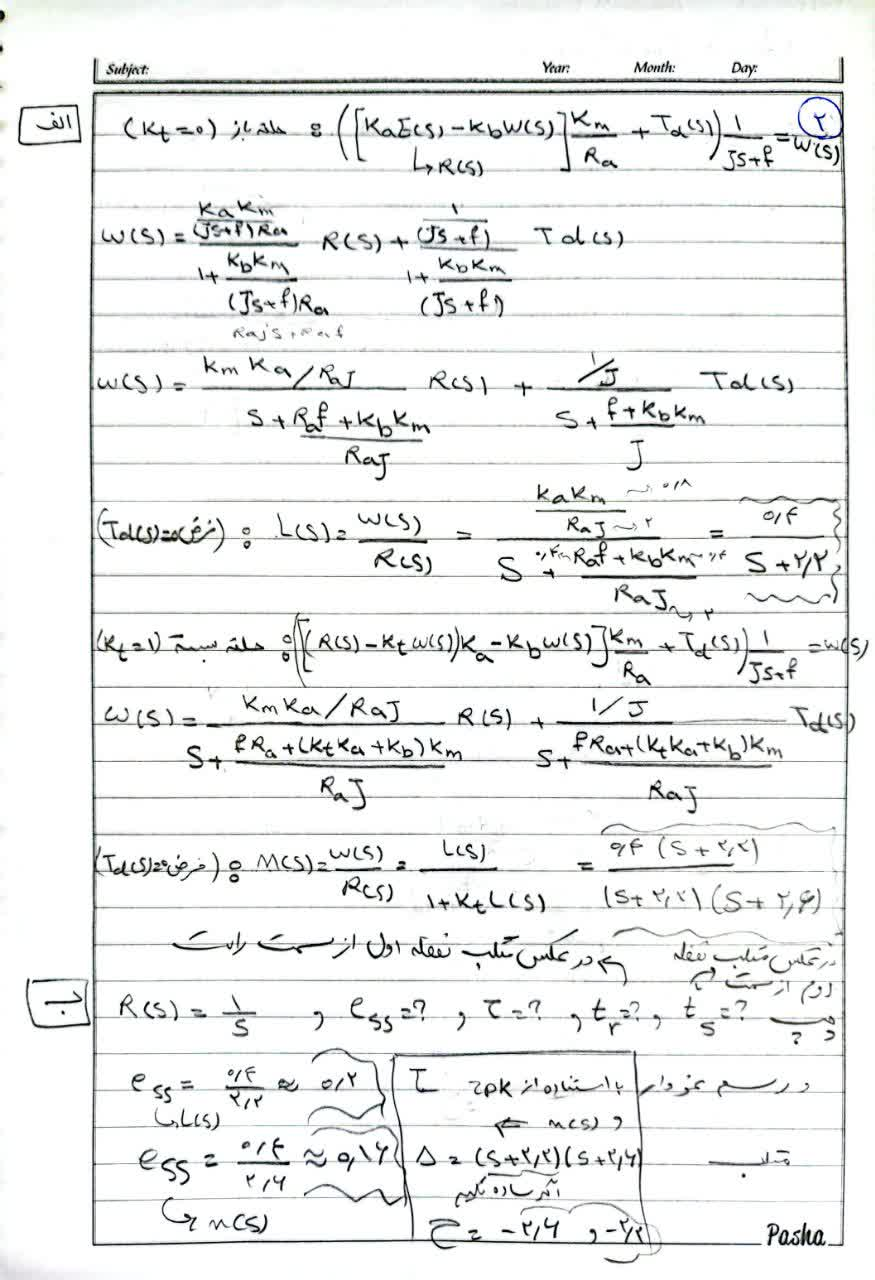
\includegraphics[width=15cm]{h2s2.jpg}\\
			
			%    \end{figure}
		
		\section{سوال سوم}{
			%    \begin{figure}
				%    	\textbf{سوال 3 :}
				%    	\centering
				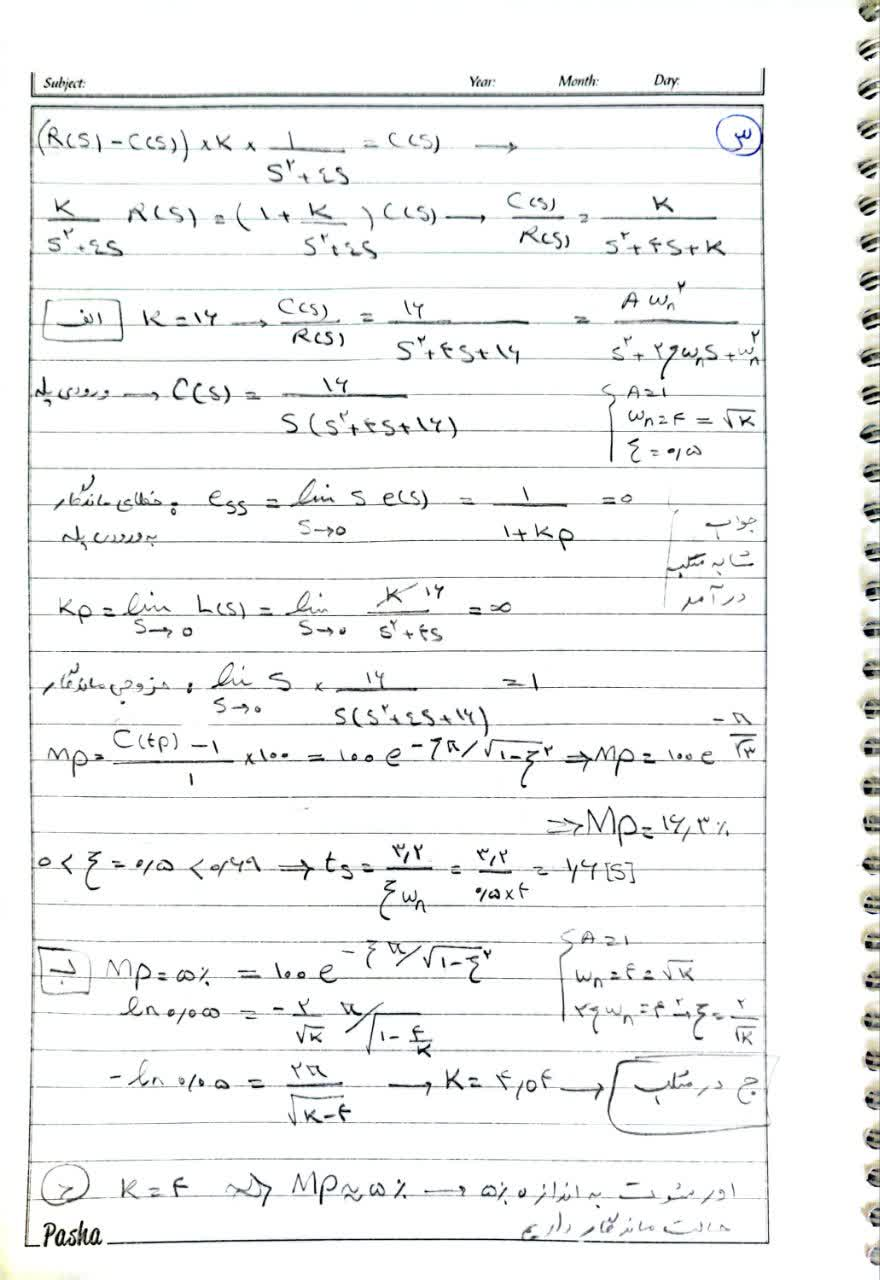
\includegraphics[width=15cm]{h2s3.jpg}
				
				
				%   \end{figure}
		}
		
		\section{سوال چهارم}{
			%    \begin{figure}
				%    	\textbf{سوال 4 :}   	
				%    	\centering
				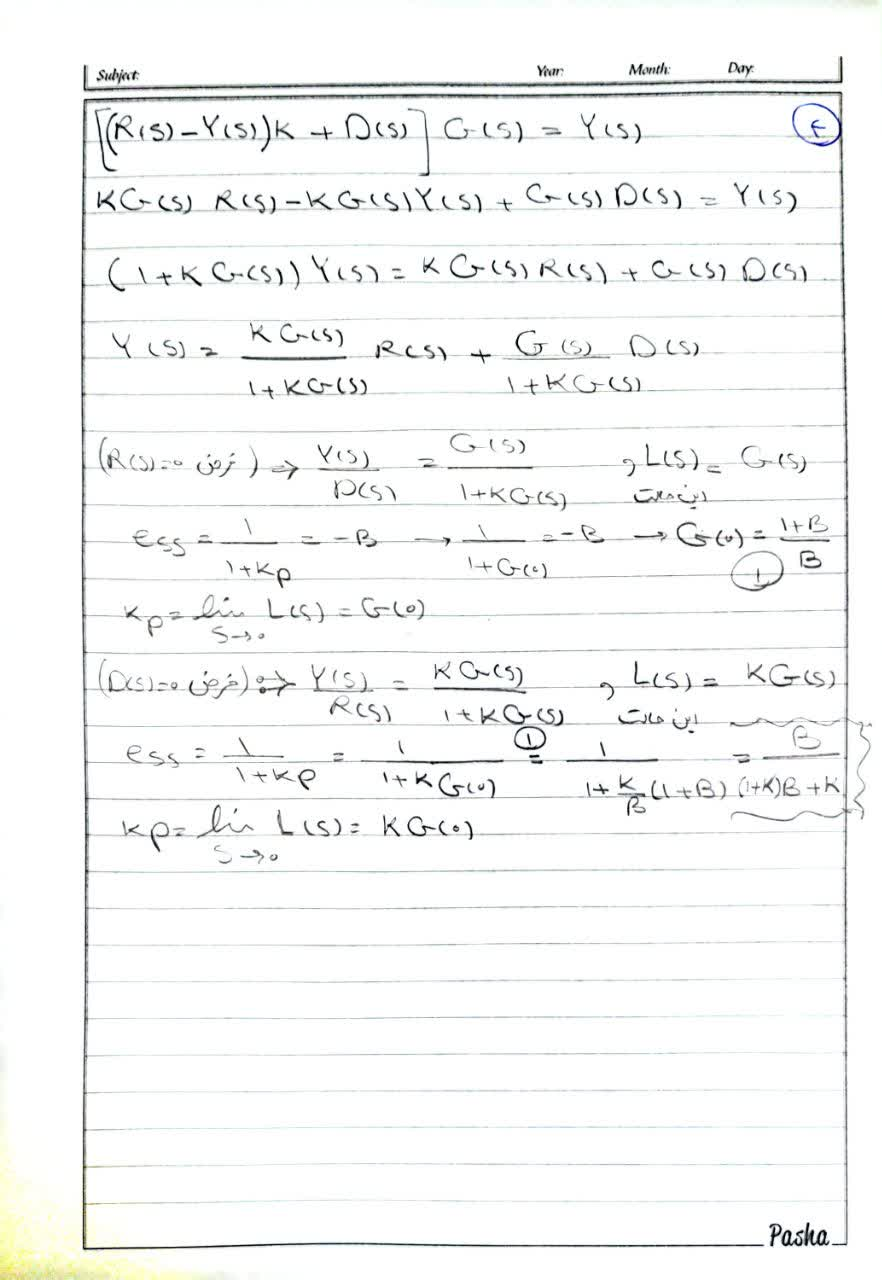
\includegraphics[width=15cm]{h2s4.jpg}
				%    \end{figure}
		}
		\section{سوال پنجم}{
			%    \begin{figure}
				%    	\textbf{سوال 4 :}   	
				%    	\centering
				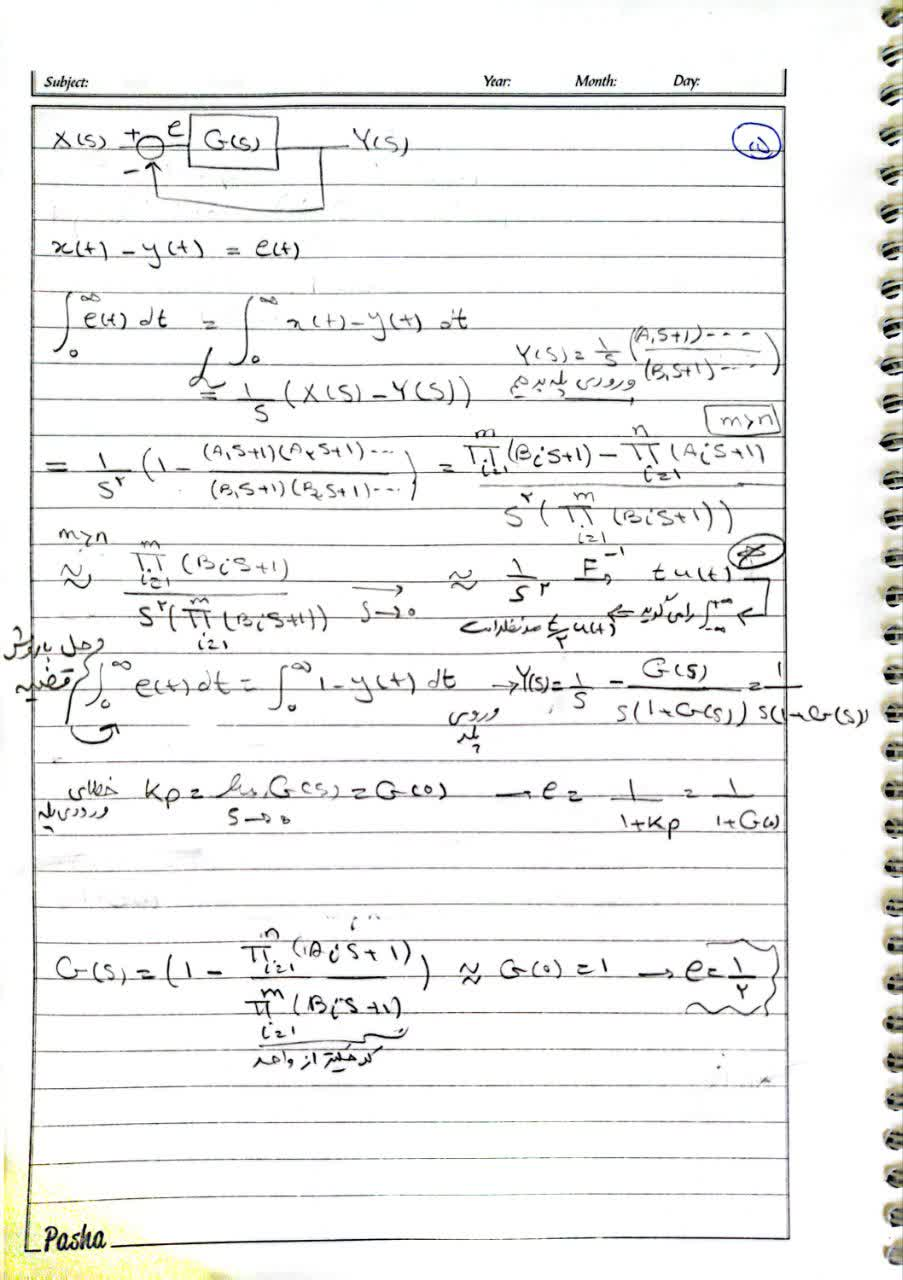
\includegraphics[width=15cm]{h2s5.jpg}
				%    \end{figure}
		}
	\end{document}
	
